% Options for packages loaded elsewhere
\PassOptionsToPackage{unicode}{hyperref}
\PassOptionsToPackage{hyphens}{url}
\PassOptionsToPackage{dvipsnames,svgnames,x11names}{xcolor}
%
\documentclass[
  letterpaper,
  DIV=11,
  numbers=noendperiod]{scrartcl}

\usepackage{amsmath,amssymb}
\usepackage{iftex}
\ifPDFTeX
  \usepackage[T1]{fontenc}
  \usepackage[utf8]{inputenc}
  \usepackage{textcomp} % provide euro and other symbols
\else % if luatex or xetex
  \usepackage{unicode-math}
  \defaultfontfeatures{Scale=MatchLowercase}
  \defaultfontfeatures[\rmfamily]{Ligatures=TeX,Scale=1}
\fi
\usepackage{lmodern}
\ifPDFTeX\else  
    % xetex/luatex font selection
\fi
% Use upquote if available, for straight quotes in verbatim environments
\IfFileExists{upquote.sty}{\usepackage{upquote}}{}
\IfFileExists{microtype.sty}{% use microtype if available
  \usepackage[]{microtype}
  \UseMicrotypeSet[protrusion]{basicmath} % disable protrusion for tt fonts
}{}
\makeatletter
\@ifundefined{KOMAClassName}{% if non-KOMA class
  \IfFileExists{parskip.sty}{%
    \usepackage{parskip}
  }{% else
    \setlength{\parindent}{0pt}
    \setlength{\parskip}{6pt plus 2pt minus 1pt}}
}{% if KOMA class
  \KOMAoptions{parskip=half}}
\makeatother
\usepackage{xcolor}
\setlength{\emergencystretch}{3em} % prevent overfull lines
\setcounter{secnumdepth}{-\maxdimen} % remove section numbering
% Make \paragraph and \subparagraph free-standing
\ifx\paragraph\undefined\else
  \let\oldparagraph\paragraph
  \renewcommand{\paragraph}[1]{\oldparagraph{#1}\mbox{}}
\fi
\ifx\subparagraph\undefined\else
  \let\oldsubparagraph\subparagraph
  \renewcommand{\subparagraph}[1]{\oldsubparagraph{#1}\mbox{}}
\fi

\usepackage{color}
\usepackage{fancyvrb}
\newcommand{\VerbBar}{|}
\newcommand{\VERB}{\Verb[commandchars=\\\{\}]}
\DefineVerbatimEnvironment{Highlighting}{Verbatim}{commandchars=\\\{\}}
% Add ',fontsize=\small' for more characters per line
\usepackage{framed}
\definecolor{shadecolor}{RGB}{241,243,245}
\newenvironment{Shaded}{\begin{snugshade}}{\end{snugshade}}
\newcommand{\AlertTok}[1]{\textcolor[rgb]{0.68,0.00,0.00}{#1}}
\newcommand{\AnnotationTok}[1]{\textcolor[rgb]{0.37,0.37,0.37}{#1}}
\newcommand{\AttributeTok}[1]{\textcolor[rgb]{0.40,0.45,0.13}{#1}}
\newcommand{\BaseNTok}[1]{\textcolor[rgb]{0.68,0.00,0.00}{#1}}
\newcommand{\BuiltInTok}[1]{\textcolor[rgb]{0.00,0.23,0.31}{#1}}
\newcommand{\CharTok}[1]{\textcolor[rgb]{0.13,0.47,0.30}{#1}}
\newcommand{\CommentTok}[1]{\textcolor[rgb]{0.37,0.37,0.37}{#1}}
\newcommand{\CommentVarTok}[1]{\textcolor[rgb]{0.37,0.37,0.37}{\textit{#1}}}
\newcommand{\ConstantTok}[1]{\textcolor[rgb]{0.56,0.35,0.01}{#1}}
\newcommand{\ControlFlowTok}[1]{\textcolor[rgb]{0.00,0.23,0.31}{#1}}
\newcommand{\DataTypeTok}[1]{\textcolor[rgb]{0.68,0.00,0.00}{#1}}
\newcommand{\DecValTok}[1]{\textcolor[rgb]{0.68,0.00,0.00}{#1}}
\newcommand{\DocumentationTok}[1]{\textcolor[rgb]{0.37,0.37,0.37}{\textit{#1}}}
\newcommand{\ErrorTok}[1]{\textcolor[rgb]{0.68,0.00,0.00}{#1}}
\newcommand{\ExtensionTok}[1]{\textcolor[rgb]{0.00,0.23,0.31}{#1}}
\newcommand{\FloatTok}[1]{\textcolor[rgb]{0.68,0.00,0.00}{#1}}
\newcommand{\FunctionTok}[1]{\textcolor[rgb]{0.28,0.35,0.67}{#1}}
\newcommand{\ImportTok}[1]{\textcolor[rgb]{0.00,0.46,0.62}{#1}}
\newcommand{\InformationTok}[1]{\textcolor[rgb]{0.37,0.37,0.37}{#1}}
\newcommand{\KeywordTok}[1]{\textcolor[rgb]{0.00,0.23,0.31}{#1}}
\newcommand{\NormalTok}[1]{\textcolor[rgb]{0.00,0.23,0.31}{#1}}
\newcommand{\OperatorTok}[1]{\textcolor[rgb]{0.37,0.37,0.37}{#1}}
\newcommand{\OtherTok}[1]{\textcolor[rgb]{0.00,0.23,0.31}{#1}}
\newcommand{\PreprocessorTok}[1]{\textcolor[rgb]{0.68,0.00,0.00}{#1}}
\newcommand{\RegionMarkerTok}[1]{\textcolor[rgb]{0.00,0.23,0.31}{#1}}
\newcommand{\SpecialCharTok}[1]{\textcolor[rgb]{0.37,0.37,0.37}{#1}}
\newcommand{\SpecialStringTok}[1]{\textcolor[rgb]{0.13,0.47,0.30}{#1}}
\newcommand{\StringTok}[1]{\textcolor[rgb]{0.13,0.47,0.30}{#1}}
\newcommand{\VariableTok}[1]{\textcolor[rgb]{0.07,0.07,0.07}{#1}}
\newcommand{\VerbatimStringTok}[1]{\textcolor[rgb]{0.13,0.47,0.30}{#1}}
\newcommand{\WarningTok}[1]{\textcolor[rgb]{0.37,0.37,0.37}{\textit{#1}}}

\providecommand{\tightlist}{%
  \setlength{\itemsep}{0pt}\setlength{\parskip}{0pt}}\usepackage{longtable,booktabs,array}
\usepackage{calc} % for calculating minipage widths
% Correct order of tables after \paragraph or \subparagraph
\usepackage{etoolbox}
\makeatletter
\patchcmd\longtable{\par}{\if@noskipsec\mbox{}\fi\par}{}{}
\makeatother
% Allow footnotes in longtable head/foot
\IfFileExists{footnotehyper.sty}{\usepackage{footnotehyper}}{\usepackage{footnote}}
\makesavenoteenv{longtable}
\usepackage{graphicx}
\makeatletter
\def\maxwidth{\ifdim\Gin@nat@width>\linewidth\linewidth\else\Gin@nat@width\fi}
\def\maxheight{\ifdim\Gin@nat@height>\textheight\textheight\else\Gin@nat@height\fi}
\makeatother
% Scale images if necessary, so that they will not overflow the page
% margins by default, and it is still possible to overwrite the defaults
% using explicit options in \includegraphics[width, height, ...]{}
\setkeys{Gin}{width=\maxwidth,height=\maxheight,keepaspectratio}
% Set default figure placement to htbp
\makeatletter
\def\fps@figure{htbp}
\makeatother

\KOMAoption{captions}{tableheading}
\makeatletter
\makeatother
\makeatletter
\makeatother
\makeatletter
\@ifpackageloaded{caption}{}{\usepackage{caption}}
\AtBeginDocument{%
\ifdefined\contentsname
  \renewcommand*\contentsname{Table of contents}
\else
  \newcommand\contentsname{Table of contents}
\fi
\ifdefined\listfigurename
  \renewcommand*\listfigurename{List of Figures}
\else
  \newcommand\listfigurename{List of Figures}
\fi
\ifdefined\listtablename
  \renewcommand*\listtablename{List of Tables}
\else
  \newcommand\listtablename{List of Tables}
\fi
\ifdefined\figurename
  \renewcommand*\figurename{Figure}
\else
  \newcommand\figurename{Figure}
\fi
\ifdefined\tablename
  \renewcommand*\tablename{Table}
\else
  \newcommand\tablename{Table}
\fi
}
\@ifpackageloaded{float}{}{\usepackage{float}}
\floatstyle{ruled}
\@ifundefined{c@chapter}{\newfloat{codelisting}{h}{lop}}{\newfloat{codelisting}{h}{lop}[chapter]}
\floatname{codelisting}{Listing}
\newcommand*\listoflistings{\listof{codelisting}{List of Listings}}
\makeatother
\makeatletter
\@ifpackageloaded{caption}{}{\usepackage{caption}}
\@ifpackageloaded{subcaption}{}{\usepackage{subcaption}}
\makeatother
\makeatletter
\@ifpackageloaded{tcolorbox}{}{\usepackage[skins,breakable]{tcolorbox}}
\makeatother
\makeatletter
\@ifundefined{shadecolor}{\definecolor{shadecolor}{rgb}{.97, .97, .97}}
\makeatother
\makeatletter
\makeatother
\makeatletter
\makeatother
\ifLuaTeX
  \usepackage{selnolig}  % disable illegal ligatures
\fi
\IfFileExists{bookmark.sty}{\usepackage{bookmark}}{\usepackage{hyperref}}
\IfFileExists{xurl.sty}{\usepackage{xurl}}{} % add URL line breaks if available
\urlstyle{same} % disable monospaced font for URLs
\hypersetup{
  pdftitle={TP : Support Vector Machine},
  pdfauthor={BEX Roméo},
  colorlinks=true,
  linkcolor={blue},
  filecolor={Maroon},
  citecolor={Blue},
  urlcolor={Blue},
  pdfcreator={LaTeX via pandoc}}

\title{TP : Support Vector Machine}
\author{BEX Roméo}
\date{2024-09-24}

\begin{document}
\maketitle
\ifdefined\Shaded\renewenvironment{Shaded}{\begin{tcolorbox}[breakable, frame hidden, borderline west={3pt}{0pt}{shadecolor}, interior hidden, boxrule=0pt, enhanced, sharp corners]}{\end{tcolorbox}}\fi

\begin{figure}

{\centering 
\includegraphics[width=0.3\textwidth,height=\textheight]{tp_files/mediabag/logo_um.pdf}

}

\caption{-}

\end{figure}

\hypertarget{introduction}{%
\section{Introduction}\label{introduction}}

Dans ce rapport, nous présentons une étude sur l'application des
\textbf{SVM} (Machines à Vecteurs de Support) pour la classification de
données. Nous abordons plusieurs aspects, tels que l'impact des noyaux
linéaires et polynomiaux, l'ajout de variables de nuisance, et la
réduction de dimension avec PCA.

Mathématiquement, Le modèle SVM optimise la fonction suivante : \[ 
\underset{\mathbf{w},b}{argmin} \left( \frac{1}{2} ||\mathbf{w}||^2 \right) + C \sum_{i=1}^{n} \max(0, 1 - y_i(\mathbf{w} \cdot \mathbf{x}_i + b))
\]

Le paramètre \textbf{C} contrôle le compromis entre la maximisation de
la marge et la réduction des erreurs de classification sur les données
d'entraînement.

Les algorithmes sont testés sur des jeux de données tels que
\textbf{Iris} et \textbf{Labeled Faces in the Wild (LFW)}.

\hypertarget{question-1}{%
\subsection{Question 1 :}\label{question-1}}

Nous appliquons un SVM à noyau linéaire sur l'ensemble de données Iris
avec lequel on fait une recherche par grille pour optimiser le paramètre
de régularisation C.

\begin{Shaded}
\begin{Highlighting}[]
\CommentTok{\# Définir les paramètres pour la recherche de grille}
\NormalTok{parameters }\OperatorTok{=}\NormalTok{ \{}\StringTok{\textquotesingle{}kernel\textquotesingle{}}\NormalTok{: [}\StringTok{\textquotesingle{}linear\textquotesingle{}}\NormalTok{], }\StringTok{\textquotesingle{}C\textquotesingle{}}\NormalTok{: }\BuiltInTok{list}\NormalTok{(np.logspace(}\OperatorTok{{-}}\DecValTok{3}\NormalTok{, }\DecValTok{3}\NormalTok{, }\DecValTok{200}\NormalTok{))\}}

\CommentTok{\# Utiliser GridSearchCV pour optimiser le modèle SVM avec noyau linéaire}
\NormalTok{clf\_linear }\OperatorTok{=}\NormalTok{ GridSearchCV(SVC(), parameters, n\_jobs}\OperatorTok{=}\DecValTok{1}\NormalTok{)}
\NormalTok{clf\_linear.fit(X\_train, y\_train)  }\CommentTok{\# Entraînement du modèle}

\CommentTok{\# Calculer les scores de généralisation et les afficher}
\NormalTok{train\_score }\OperatorTok{=}\NormalTok{ clf\_linear.score(X\_train, y\_train)}
\NormalTok{test\_score }\OperatorTok{=}\NormalTok{ clf\_linear.score(X\_test, y\_test)}
\BuiltInTok{print}\NormalTok{(}\SpecialStringTok{f\textquotesingle{}Generalization score for linear kernel: }\SpecialCharTok{\{}\NormalTok{train\_score}\SpecialCharTok{\}}\SpecialStringTok{, }\SpecialCharTok{\{}\NormalTok{test\_score}\SpecialCharTok{\}}\SpecialStringTok{\textquotesingle{}}\NormalTok{)}
\end{Highlighting}
\end{Shaded}

\textbf{Renvoie en sortie :}

\begin{itemize}
\tightlist
\item
  Précision sur l'ensemble de test 0.62
\item
  Précision sur l'ensemble d'entraînement : 0.72
\end{itemize}

\hypertarget{question-2}{%
\subsection{Question 2 :}\label{question-2}}

Nous appliquons cette fois un SVM à noyau polynomial.

\begin{Shaded}
\begin{Highlighting}[]
\CommentTok{\# Définir les paramètres pour le noyau polynomial}
\NormalTok{Cs }\OperatorTok{=} \BuiltInTok{list}\NormalTok{(np.logspace(}\OperatorTok{{-}}\DecValTok{3}\NormalTok{, }\DecValTok{3}\NormalTok{, }\DecValTok{5}\NormalTok{))}
\NormalTok{gammas }\OperatorTok{=} \FloatTok{10.} \OperatorTok{**}\NormalTok{ np.arange(}\DecValTok{1}\NormalTok{, }\DecValTok{2}\NormalTok{)}
\NormalTok{degrees }\OperatorTok{=}\NormalTok{ np.r\_[}\DecValTok{1}\NormalTok{, }\DecValTok{2}\NormalTok{, }\DecValTok{3}\NormalTok{]}

\NormalTok{parameters }\OperatorTok{=}\NormalTok{ \{}\StringTok{\textquotesingle{}kernel\textquotesingle{}}\NormalTok{: [}\StringTok{\textquotesingle{}poly\textquotesingle{}}\NormalTok{], }\StringTok{\textquotesingle{}C\textquotesingle{}}\NormalTok{: Cs, }\StringTok{\textquotesingle{}gamma\textquotesingle{}}\NormalTok{: gammas, }\StringTok{\textquotesingle{}degree\textquotesingle{}}\NormalTok{: degrees\}}

\CommentTok{\# Utiliser GridSearchCV pour optimiser le modèle SVM avec noyau polynomial}
\NormalTok{clf\_poly }\OperatorTok{=}\NormalTok{ GridSearchCV(SVC(), parameters, cv}\OperatorTok{=}\DecValTok{5}\NormalTok{)}
\NormalTok{clf\_poly.fit(X\_train, y\_train)}

\CommentTok{\# Afficher les meilleurs paramètres}
\BuiltInTok{print}\NormalTok{(clf\_poly.best\_params\_)}
\end{Highlighting}
\end{Shaded}

On obtient alors en sortie :

\begin{itemize}
\tightlist
\item
  \texttt{C} : 0.031
\item
  Degré (polynôme) : 1
\item
  Gamma : 10.0
\end{itemize}

Avec comme score de généralisation de 0.71 (pour les donnés
d'entraînement) et 0.68 pour (pour les donnés tests)

\begin{figure}

{\centering 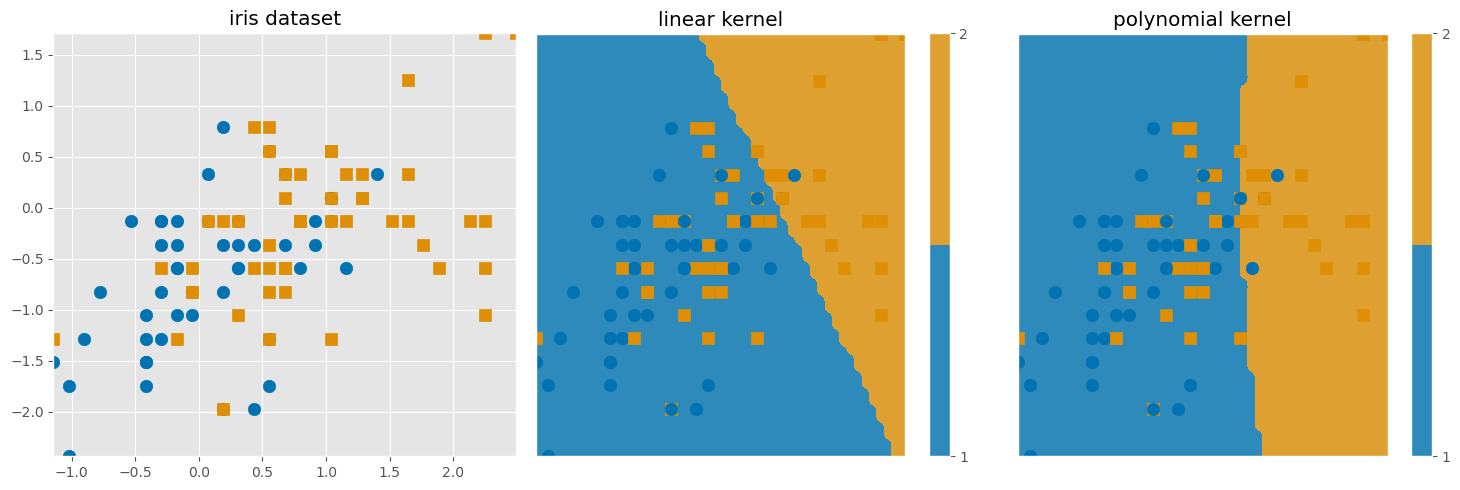
\includegraphics[width=0.8\textwidth,height=\textheight]{tp_files/mediabag/bg.pdf}

}

\caption{Frontière de décision des noyaux linéaire et polynomial}

\end{figure}

\hypertarget{question-3-bonus}{%
\subsection{Question 3 (bonus) :}\label{question-3-bonus}}

Nous allons optimiser le paramètre \texttt{C} avec SVM linéaire sur le
jeu de donnée de visages fournis à l'adresse indiqué. En voici un
extrait imagé :

\begin{figure}

{\centering 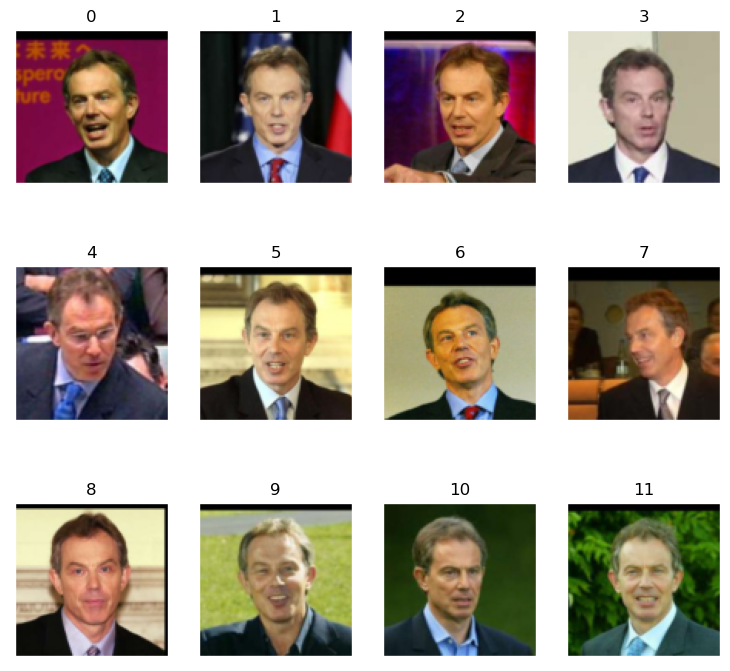
\includegraphics[width=0.6\textwidth,height=\textheight]{tp_files/mediabag/extraits.pdf}

}

\caption{Labeled Faces in the Wild (LFW).}

\end{figure}

Pour ça on utilisera \texttt{GridSearchCV} pour tester plusieurs
variables de \texttt{C}.

\begin{Shaded}
\begin{Highlighting}[]
\NormalTok{Cs }\OperatorTok{=} \FloatTok{10.} \OperatorTok{**}\NormalTok{ np.arange(}\OperatorTok{{-}}\DecValTok{5}\NormalTok{, }\DecValTok{6}\NormalTok{)}
\NormalTok{scores }\OperatorTok{=}\NormalTok{ []}
\ControlFlowTok{for}\NormalTok{ C }\KeywordTok{in}\NormalTok{ Cs:}
\NormalTok{    clf }\OperatorTok{=}\NormalTok{ SVC(kernel}\OperatorTok{=}\StringTok{\textquotesingle{}linear\textquotesingle{}}\NormalTok{, C}\OperatorTok{=}\NormalTok{C)}
\NormalTok{    clf.fit(X\_train, y\_train)}
\NormalTok{    scores.append(clf.score(X\_test, y\_test))}

\CommentTok{\# Meilleur C et graphique des scores}
\NormalTok{best\_C }\OperatorTok{=}\NormalTok{ Cs[np.argmax(scores)]}
\NormalTok{plt.plot(Cs, scores)}
\NormalTok{plt.xscale(}\StringTok{\textquotesingle{}log\textquotesingle{}}\NormalTok{)}
\NormalTok{plt.title(}\SpecialStringTok{f"Optimisation du paramètre C"}\NormalTok{)}
\NormalTok{plt.show()}

\BuiltInTok{print}\NormalTok{(}\SpecialStringTok{f"Meilleur paramètre C : }\SpecialCharTok{\{}\NormalTok{best\_C}\SpecialCharTok{\}}\SpecialStringTok{"}\NormalTok{)}
\BuiltInTok{print}\NormalTok{(}\SpecialStringTok{f"Meilleur score: }\SpecialCharTok{\{}\NormalTok{np}\SpecialCharTok{.}\BuiltInTok{max}\NormalTok{(scores)}\SpecialCharTok{\}}\SpecialStringTok{"}\NormalTok{)}
\end{Highlighting}
\end{Shaded}

On trouve comme résultat en sortie une \textbf{accuracy} d'environ 0.95
cela indique que le modèle est bien capable de généraliser les données
de test.

De plus si \texttt{C} est petit :

\begin{itemize}
\tightlist
\item
  Cela peut entraîner du sous-apprentissage (underfitting) car le modèle
  devient trop simple et risque de ne pas capturer suffisamment
  l'ensemble des données et ce la peut se traduire par une acuracy plus
  faible.
\item
  On aperçoit alors une baisse de la performance du modèle.
\end{itemize}

\hypertarget{question-4}{%
\subsection{Question 4 :}\label{question-4}}

\begin{figure}

{\centering \includegraphics[width=0.6\textwidth,height=\textheight]{tp_files/mediabag/graphique_scores_svm.pdf}

}

\caption{Graphique de Scores d'Apprentissage}

\end{figure}

Le modèle se comporte de manière optimale avec un C autour de de
\(10^{-2}\) à \(10^2\), où il atteint un score d'environ 0.95. Pour des
valeurs de C trop petites, le modèle sous-apprend, tandis que pour des
valeurs très élevées de C, le modèle ne montre pas de sur-apprentissage,
mais n'améliore pas non plus ses performances.

\hypertarget{question-5}{%
\subsection{Question 5 :}\label{question-5}}

Nous avons ajouter des variables de nuisances (250) aux données pour
étudier l'impact du bruit sur les performances du modèle.

\begin{Shaded}
\begin{Highlighting}[]
\CommentTok{\# Ajout de 250 variables de nuisance}
\NormalTok{noise }\OperatorTok{=}\NormalTok{ sigma }\OperatorTok{*}\NormalTok{ np.random.randn(n\_samples, }\DecValTok{250}\NormalTok{)}
\NormalTok{X\_noisy }\OperatorTok{=}\NormalTok{ np.concatenate((X, noise), axis}\OperatorTok{=}\DecValTok{1}\NormalTok{)}
\NormalTok{X\_noisy }\OperatorTok{=}\NormalTok{ X\_noisy[np.random.permutation(X.shape[}\DecValTok{0}\NormalTok{])]}

\CommentTok{\# Validation croisée avec bruit}
\NormalTok{run\_svm\_cv(X\_noisy, y)}
\end{Highlighting}
\end{Shaded}

Sans bruit, le modèle SVM obtenait une accuracy d'environ 95\%. Après
ajout du bruit, l'accuracy est tombée à 52\%, ce qui montre l'importance
d'éliminer les variables non pertinentes.

\hypertarget{question-6}{%
\subsection{Question 6 :}\label{question-6}}

\begin{Shaded}
\begin{Highlighting}[]
\CommentTok{\# Réduction de dimension avec PCA}
\NormalTok{n\_components }\OperatorTok{=} \DecValTok{20}
\NormalTok{pca }\OperatorTok{=}\NormalTok{ PCA(n\_components}\OperatorTok{=}\NormalTok{n\_components, svd\_solver}\OperatorTok{=}\StringTok{\textquotesingle{}randomized\textquotesingle{}}\NormalTok{).fit(X\_noisy)}
\NormalTok{X\_reduced }\OperatorTok{=}\NormalTok{ pca.transform(X\_noisy)}

\CommentTok{\# Validation croisée sur les données réduites}
\NormalTok{run\_svm\_cv(X\_reduced, y)}
\end{Highlighting}
\end{Shaded}

Pour améliorer les performances en présence de bruit, nous avons
appliqué une réduction de dimension à l'aide de l'algorithme PCA avec le
solveur \texttt{randomized}.



\end{document}
